\documentclass[12pt]{article}
\usepackage{xeCJK}%preamble part
\usepackage{graphicx}
\usepackage{multirow}
\usepackage{indentfirst}
\usepackage[a4paper, inner=1.5cm, outer=3cm, top=2cm, bottom=3cm, bindingoffset=1cm]{geometry}
\usepackage{epstopdf}
\usepackage{listings}
\usepackage{array}
\usepackage{color}
\usepackage{fontspec}
\usepackage{caption}
\usepackage{subcaption}
\usepackage{bm}
\usepackage{gensymb}
\usepackage{todonotes}
\usepackage{amsmath, amsthm, amssymb}
\usepackage[citecolor=blue]{hyperref}
\newtheorem{definition}{Definition}
\newtheorem{thm}{Theorem}[section]
\newtheorem{cor}[thm]{Corollary}
\newtheorem{lem}[thm]{Lemma}
\DeclareMathOperator{\sgn}{sgn}
\theoremstyle{remark}
\newtheorem*{rem}{Remark}
\usepackage{makecell}
\setCJKmainfont[BoldFont={SimHei}]{SimSun}
\setCJKmonofont{SimSun}
\setmainfont{Times New Roman}
\newCJKfontfamily[hei]\heiti{SimHei}
\setlength{\extrarowheight}{4pt}
\setlength{\parindent}{1cm}
\definecolor{codegreen}{rgb}{0,0.6,0}
\definecolor{codegray}{rgb}{0.5,0.5,0.5}
\definecolor{codepurple}{rgb}{0.58,0,0.82}
\definecolor{backcolour}{rgb}{0.95,0.95,0.92}
\lstdefinestyle{mystyle}{
    backgroundcolor=\color{backcolour},   
    commentstyle=\color{codegreen},
    keywordstyle=\color{magenta},
    numberstyle=\tiny\color{codegray},
    stringstyle=\color{codepurple},
    basicstyle=\footnotesize,
    breakatwhitespace=false,         
    breaklines=true,                 
    captionpos=b,                    
    keepspaces=true,                 
    numbers=left,                    
    numbersep=5pt,                  
    showspaces=false,                
    showstringspaces=false,
    showtabs=false,                  
    tabsize=2
}
 
\lstset{style=mystyle}
\begin{document}
\title{\textbf{\fontsize{15.75pt}{\baselineskip}{双曲守恒律问题的差分方法实验题}}} 
\author{\fontsize{12pt}{\baselineskip}{数33 赵丰 \thanks{学号:2013012178} }}
\maketitle
\large
\section{题目}
考虑以下Burgers'方程的初值问题
\begin{equation}
\begin{cases}
\frac{\partial u}{\partial t}+\frac{\partial}{\partial x}(\frac{u^2}{2})&=0\\
u(x,0)&=u_0(x),
\end{cases}
\end{equation}
取以下初值:
\begin{equation}
u_0(x)=\begin{cases}
1,&x \in [0.4,0.6],\\
0&x \notin [0.4,0.6]
\end{cases}
\end{equation}
进行计算,算到$T=0.5$,对于适中的网格比,初值取$x \in [0,1]$进行计算。
\section{解析解}
当$t\leq 0.4$时,
\[
u(x,t)=\begin{cases}
0,&x\leq 0.4;\\
\frac{x-0.4}{t},&0.4<x<t+0.4\\
1,&t+0.4\leq x \leq 0.6+\frac{t}{2}\\
0,&x>0.6+\frac{t}{2}\\
\end{cases}
\]
当$t>0.4$时,
\[
u(x,t)=\begin{cases}
0,&x\leq 0.4 \\
\frac{x-0.4}{t},&0.4<x<0.4+\sqrt{0.4t}\\
0,&x\geq 0.4+\sqrt{0.4t}
\end{cases}
\]
\section{使用的差分格式}
本次计算使用的差分格式都是守恒型的差分格式,其具有以下基本形式:
\begin{equation}
u^{n+1}_j=u^n_j-\lambda(g^n_{j+\frac{1}{2}}-g^n_{j-\frac{1}{2}})
\end{equation}
为记号简便,设$f(u)=\frac{u^2}{2}$
\subsection{Godunov格式}
设Riemann问题的解可以写成$u(x,t)\equiv R(\frac{x}{t};u_,u_R)$的形式。
则
\begin{equation}
g^n_{j+\frac{1}{2}}=f(R(0;u^n_j,u^n_{j+1}))
\end{equation}
对于所求解的问题,Godunov格式实际上是迎风格式。
\subsection{Lax-Wendroff 格式}
\begin{equation}
g^n_{j+\frac{1}{2}}=\frac{f(u^n_j)+f(u^n_{j+1})}{2}-\frac{\lambda}{2}a^n_{j+\frac{1}{2}}(f(u^n_{j+1})-f(u^n_j))
\end{equation}

其中$\lambda=\frac{\tau}{h}$为网格比,而$a^n_{j+\frac{1}{2}}$为:
\begin{equation}
a^n_{j+\frac{1}{2}}=f'(\frac{u^n_j+u^n_{j+1}}{2})
\end{equation}

\subsection{通量限制器给出的二阶TVD格式}
迎风格式给出的数值通量记为$g^n_{L,j+\frac{1}{2}}$,
对于所求解的问题,$g^n_{L,j+\frac{1}{2}}=f(u^n_j)$
。L-W格式给出的数值通量记为$g^n_{H,j+\frac{1}{2}}$,
利用上面两种格式可以构造一个二阶的格式为
\begin{equation}
g^n_{j+\frac{1}{2}}=g^n_{L,j+\frac{1}{2}}+\phi^n_j(g^n_{H,j+\frac{1}{2}}-g^n_{L,j+\frac{1}{2}})
\end{equation}
其中$\phi_j^n=\phi(\theta_j^n)$,$\phi(\theta)$取Super Bee Limiter:
\begin{equation}
\phi(\theta)=\frac{|\theta|+\theta}{1+|\theta|}
\end{equation}
$\theta_j^n$的定义为:
\begin{equation}
\theta^n_j=\Bigg\{\begin{array}{cc}
\frac{u^n_j-u^n_{j-1}}{u^n_{j+1}-u^n_j},&a>0;\\
\frac{u^n_{j+2}-u^n_{j+1}}{u^n_{j+1}-u^n_j},&a\leq 0;
\end{array}
\end{equation}
\subsection{不同差分格式理论性能比较}
\section{数值结果}
用如上列出的数值格式分别求解给定的双曲问题,matlab代码如下:
\lstinputlisting[language=Matlab]{hyperbolic.m}
\section{结果展示}
分别取网格比$\lambda$为0.5和0.9,空间步长h为0.01和0.001用三种格式计算,得到分别在t=0.3和0.5的函数图像,取\[
\text{mse}=\sqrt{\sum_{i=1}^n (u(x_i,t)-u^*(x_i,t))^2}\]
作为误差衡量标准,
数值结果如下表所示:
\begin{table*}[!ht]
\centering
\begin{tabular}{|l|l|ccc|}
\hline
$\lambda=0.5$&&Godonov&lax\_wandroff&2TVD\\
\hline
\multirow{2}{*}{h=0.01}&t=0.3&0.44&1.55&0.30\\
&t=0.5&0.80&2.02&0.53\\
\hline
\multirow{2}{*}{h=0.001}&t=0.3&0.384&4.661&0.296\\
&t=0.5&0.777&5.997&0.204\\
\hline
\end{tabular}
\begin{tabular}{|l|l|ccc|}
\hline
$\lambda=0.9$&&Godonov&lax\_wandroff&2TVD\\
\hline
\multirow{2}{*}{h=0.01}&t=0.3&0.60&1.39&0.62\\
&t=0.5&0.85&1.72&0.81\\
\hline
\multirow{2}{*}{h=0.001}&t=0.3&0.58&3.74&0.61\\
&t=0.5&0.70&4.77&0.46\\
\hline
\end{tabular}
\end{table*}
\section{结果分析}
由于题目的特殊性,$R(0;u^n_j,u^n_{j+1})=u^n_j$,因此Godonov格式实际上是迎风格式,用lax\_wandroff
格式求解的结果随时间步的增加与解析解相差越来越大,而且减小步长并不能改善,用迎风和lax\_wandroff构造的二阶TVD格式精度比迎风格式有所提升。

分析计算结果可以看出,网格比为0.5要优于0.9的情形,
在网格比为0.9的情况下,t=0.3时使用2阶TVD计算结果的误差要比只用迎风格式来得大。

最后分别给出$\lambda=0.5$时的函数图像,由下面的图像可以看出lax\_wandroff格式不适用于解此问题。
\begin{figure}[!ht]
\centering
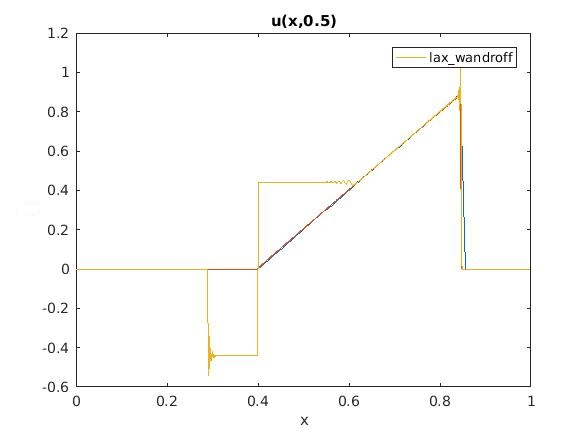
\includegraphics[width=350pt]{pde_3.jpg}
\end{figure}
\begin{figure}[!ht]
\centering
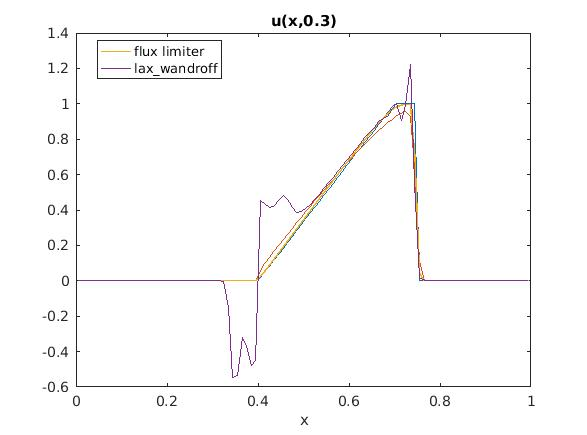
\includegraphics[width=350pt]{pde_4.jpg}
\end{figure}
\end{document}
